% !TEX root = main.tex
\chapter{Introdução}
\label{cha:intro}

\pagenumbering{arabic}
\setcounter{page}{1}



Embora o propósito deste trabalho não seja pesquisar todos os detalhes de cada área envolvida, é interessante fazer um passeio por alguns dos pontos mais importantes que ajudam a entender este problema, incluindo suas principais dificuldades e a base de como cada parte funciona. Assim, ao longo deste capítulo serão apresentados e explicados os principais conceitos, técnicas e abordagens associadas ao tema deste trabalho; uma nova abordagem também será apresentada.




%   ---------------
%   ----- BSS -----
%   ---------------
\section{Separação Cega de Fontes}
\label{sec:intro_bss}

Onde quer que estejam, os seres humanos estão sujeitos à presença de vários tipos distintos de sinais analógicos, independentemente de serem capazes de serem percebidos sem o auxílio de algum tipo de equipamento. O canto de um pássaro, os aplausos de uma multidão e as badaladas de um sino são exemplos bastante comuns que qualquer indivíduo pode vivenciar em seu dia a dia. Talvez um olhar mais científico sobre tais ocorrências tão corriqueiras seja algo incomum para a maior parte da população, porém, ainda assim, em todos os casos mencionados há muitos sinais transitando por todos os lados.

Segundo o professor Bhagwandas Pannalal Lathi,

\begin{formal}
\begin{quote}
\begin{flushright}
    \textcolor{citeblue}{\textquotedblleft \textit{A signal is a set of data or information.} \textquotedblright}\\ \citep{lathi2009linear}
\end{flushright}
\end{quote}
\end{formal}

Em uma tradução livre, segundo a citação do professor Lathi, um sinal é um conjunto de dados ou de informação. Pode parecer uma frase simples -- e, de fato, é --, mas carrega em si um significado enorme, sobretudo se forem consideradas algumas de suas implicações; trata-se, afinal, de uma definição bastante abrangente, mas bastante importante para tudo o que viria a ser futuramente desenvolvido a partir de então.

Sinais carregam informação, mas, para que um sinal seja chamado de ``informação'' usando esta nomenclatura em particular, uma dependência específica deve ser satisfeita: sua utilidade; caso contrário, poderia ser simplesmente considerado um ruído. Assim, do ponto de vista da engenharia de informação, o que permite distinguir linguisticamente um sinal puramente ruidoso de um sinal puramente informativo é a sua utilidade.

Devido à sua suscetibilidade a interferências causadas por sinais indesejados, que podem ser chamados de ruídos em alguns casos, qualquer sinal originalmente coletado da natureza traz consigo algum ruído. A origem deste ruído é irrelevante neste momento, mas suas características e a maneira como ele interfere no sinal original de informação pura são altamente relevantes, porque influencia a escolha das técnicas necessárias para filtrar o ruído \citep{tuzlukov2002signal} e um apropriado tratamento de ruído é muito importante \citep{boll1979suppression, 382009, 1451965, 4766994}. Tratamentos ineficazes podem resultar em danos aos dados, além de gastos de recursos valiosos, como tempo e energia, podendo até mesmo introduzir novos ruídos, o que só intensificaria ainda mais a complexidade do problema.


\begin{figure}[H]
    \centering
    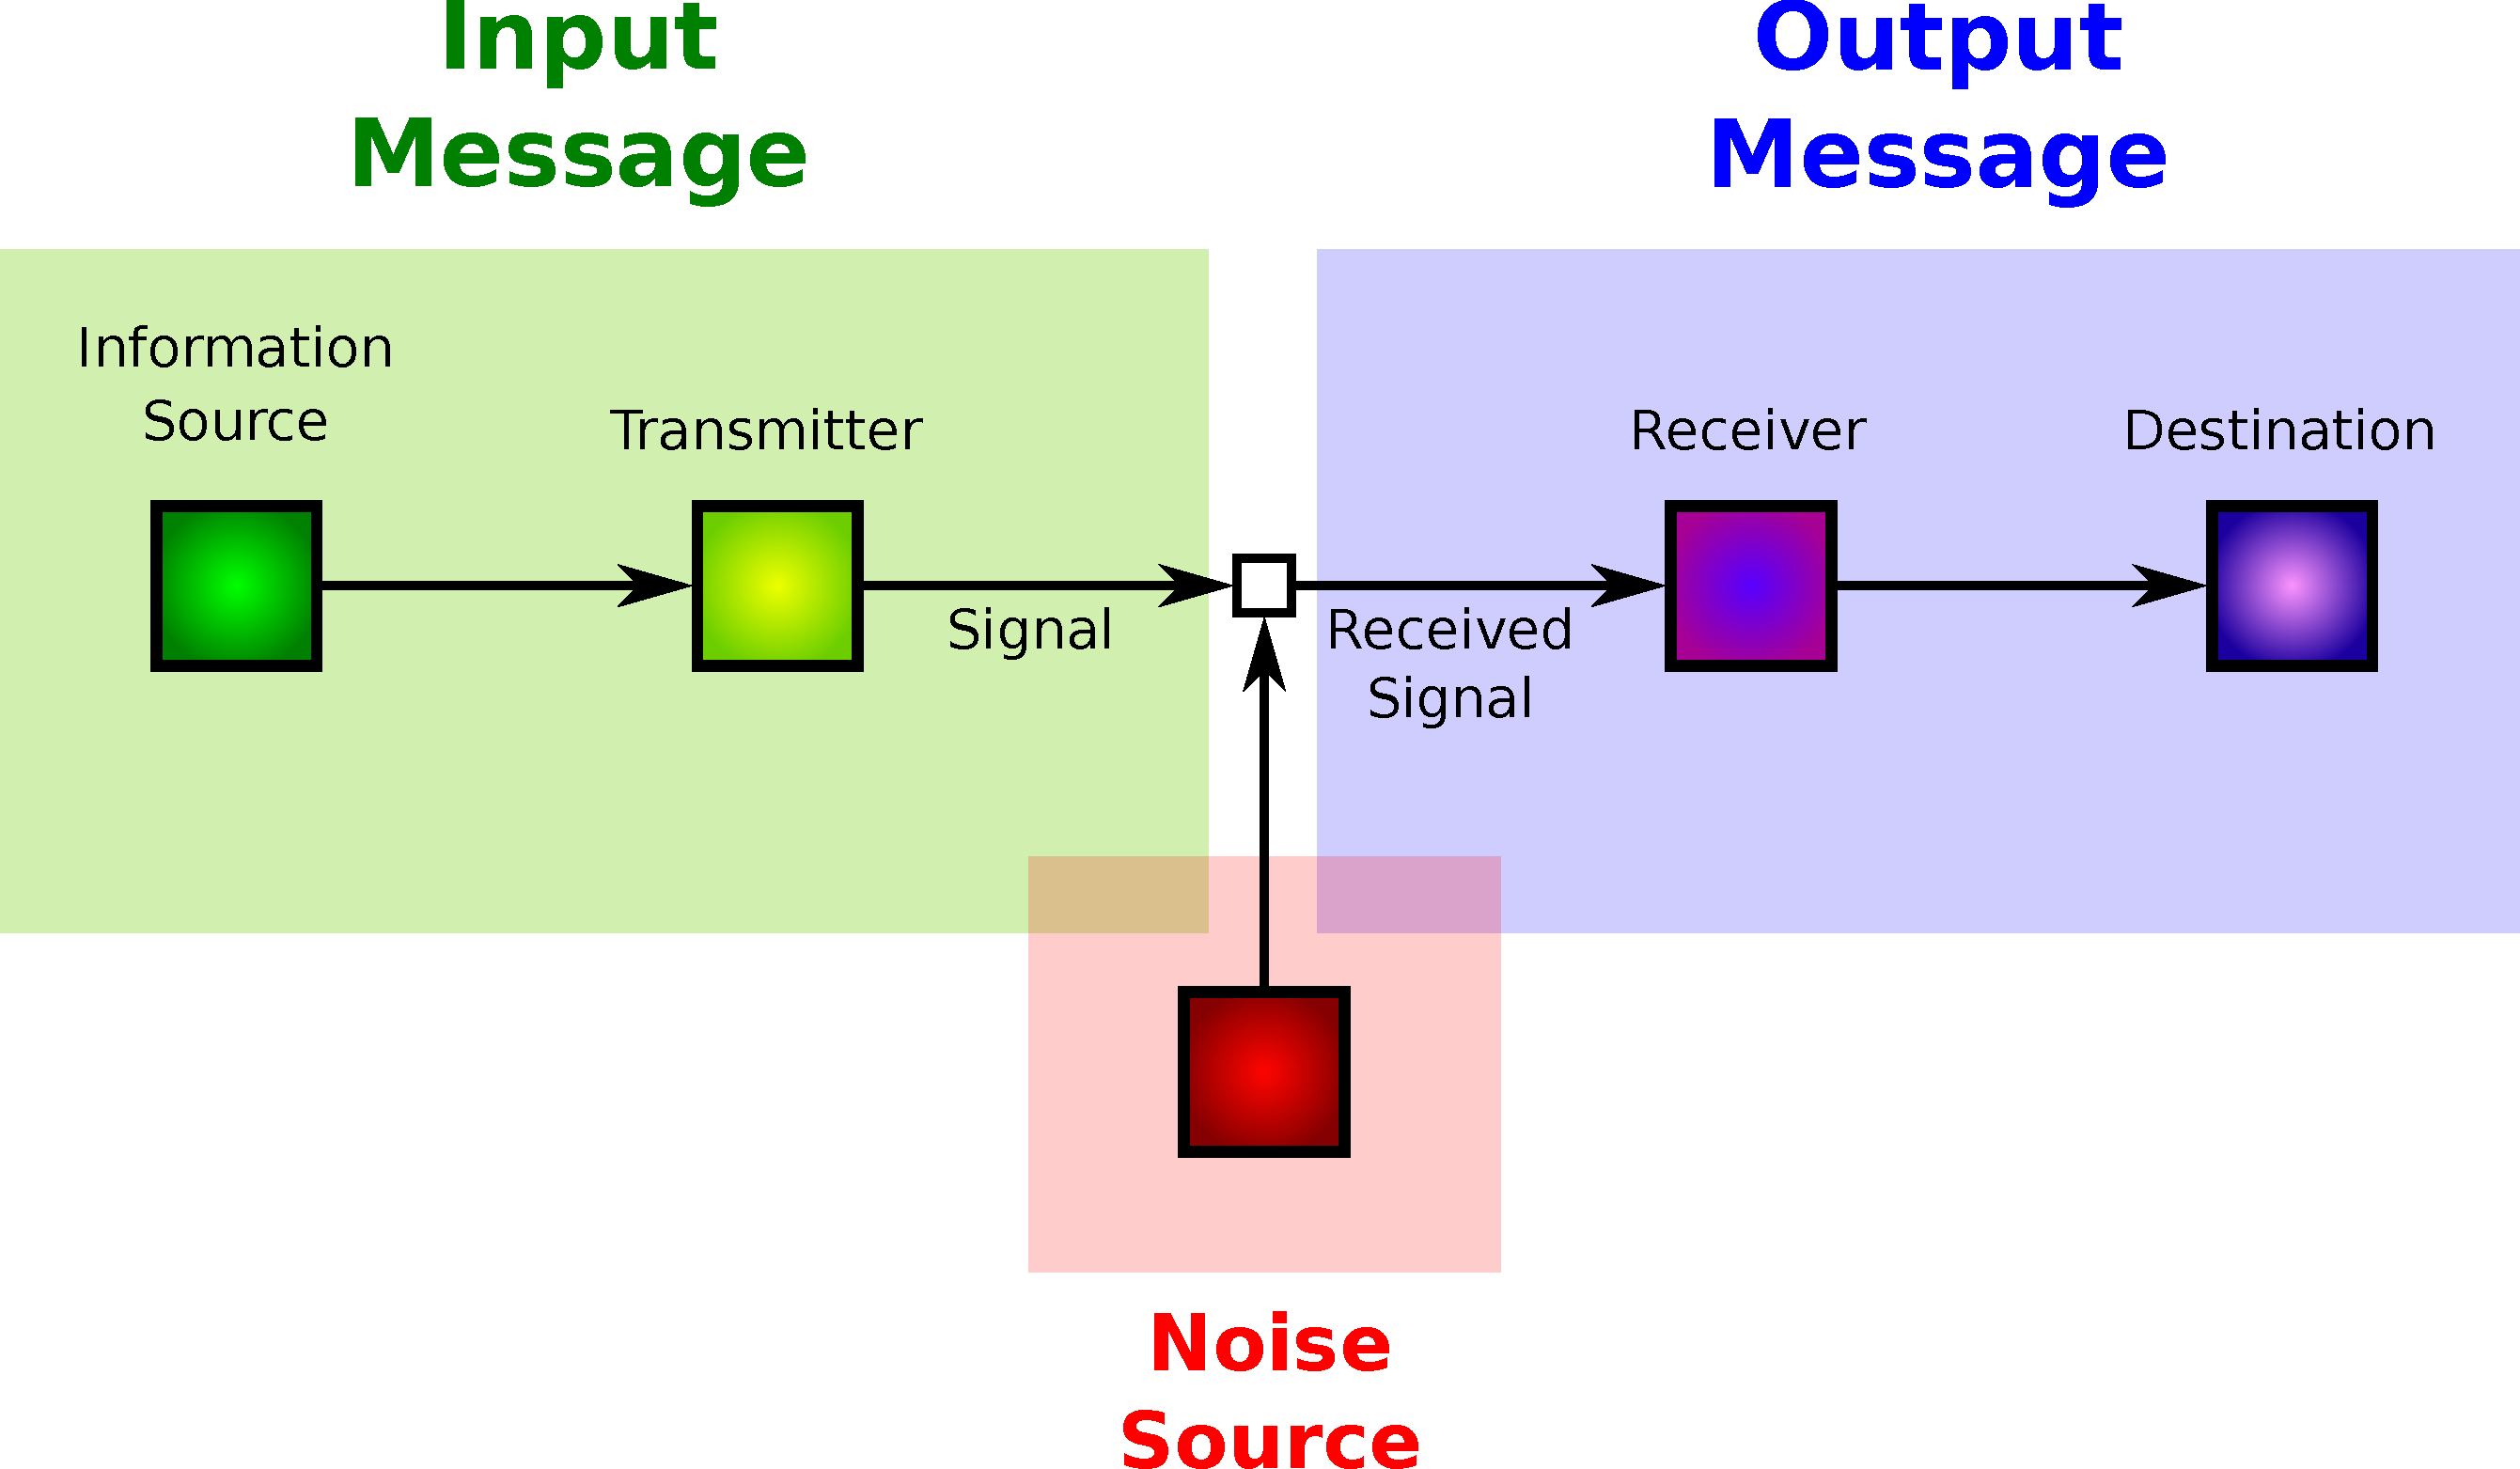
\includegraphics[width=0.75\textwidth]{figs/communication_diagram.pdf}
    \caption{Diagrama esquemático representando um sistema de comunicação, inspirado em \citep{shannon1948mathematical}.}
    \label{fig:communication_diagram}
\end{figure}

Para visualizar melhor o processo de interferência causado pelo ruído sobre o sinal de informação, veja a Figura \ref{fig:communication_diagram}. Na verdade, a versão original dessa figura foi elaborada e utilizada pelo professor Claude Elwood Shannon em um cenário focado em comunicação, mas continua sendo uma boa ilustração da ideia por detrás do problema em sua forma mais ampla.

O primeiro bloco, a Fonte de Informação (do inglês, \textit{Information Source}), representa a parte útil do sinal, o sinal original; o segundo, o Transmissor (do inglês, \textit{Transmitter}), é responsável por enviar a mensagem através do meio (canal), representado pelo pequeno quadrado branco no centro do diagrama, que pode sofrer os efeitos de múltiplos tipos de ruído; o Receptor (do inglês, \textit{Receiver}) interpreta o sinal recebido e fornece ao destino final (do inglês, \textit{Destination}) as informações obtidas. Nesta mesma figura há um bloco intitulado \textit{Noise Source}, que representa, de modo geral, todas as formas possíveis de ruído que sejam, de alguma maneira, capazes de interferir nocivamente no sinal assim que trafega ao longo do canal.

Por outro lado, há casos em que o objeto de interesse depende da separação dos sinais que estão envolvidos na composição, ou o interesse está no processo separação em si. Na literatura, há muitos bons exemplos de trabalhos que corroboram a importância de realizar uma separação de fontes, como \citep{belouchrani1997blind, nugraha2016multichannel}.

A tarefa a ser realizada para efetuar o processo de separação é conhecida como Separação de Fontes. Essa separação pode ser feita utilizando-se diversas técnicas distintas, que podem oferecer desempenhos melhores ou piores, dependendo da situação, por isso a escolha da ferramenta deve ser feita cautelosamente. Todo problema a ser atacado envolve um cenário em particular, que é um dos principais fatores a serem considerados.

De modo geral, há cinco elementos a serem considerados ao todo o processo. São eles: as fontes de origem de cada sinal, o processo de mistura que gera sinais resultantes, os sensores que registraram os sinais misturados, o processo de separação que separa os sinais misturados, e os sinais independentes já separados. Alterações, ainda que sutis, em qualquer um dos cinco elementos mencionados já pode resultar em uma mudança de cenário, o que, por sua vez, pode implicar a demanda por uma mudança de técnica para que um bom desempenho na tarefa de separação seja obtido.

Casos que envolvem fontes de sinais e processos de mistura com características inicialmente desconhecidas são tratados como pertencentes a uma categoria conhecida como ``cega'', referindo-se à falta de informações relevantes sobre as duas partes mencionadas; por isso o nome Separação Cega de Fontes (\textbf{BSS}, do inglês \textit{Blind Source Separation}). Também é comum ser utilizado o termo ``não-supervisionado'' para designar tal abordagem neste contexto. Quando se possui informações incompletas, parciais, sobre esses elementos, diz-se que se trata de uma categoria ``semi-cega'', por isso Separação Semi-Cega de Fontes (\textbf{SBSS}, do inglês \textit{Semi-Blind Source Separation}).

\nomenclature{BSS}{\textit{Blind Source Separation}}
\nomenclature{SBSS}{\textit{Semi-Blind Source Separation}}

Cabe aqui ressaltar o fato de que a separação cega de fontes é uma tarefa que não sofre limitações quanto às aplicações a que se destinam os sinais a serem separados, o que lhe confere um elevado grau de generalidade, permitindo que as ferramentas mais básicas exploradas com este mesmo objetivo possam ser utilizadas para aplicações em sinais cerebrais, música e telecomunicações, além de diversas outras áreas de aplicação.

\begin{figure}[H]
    \centering
    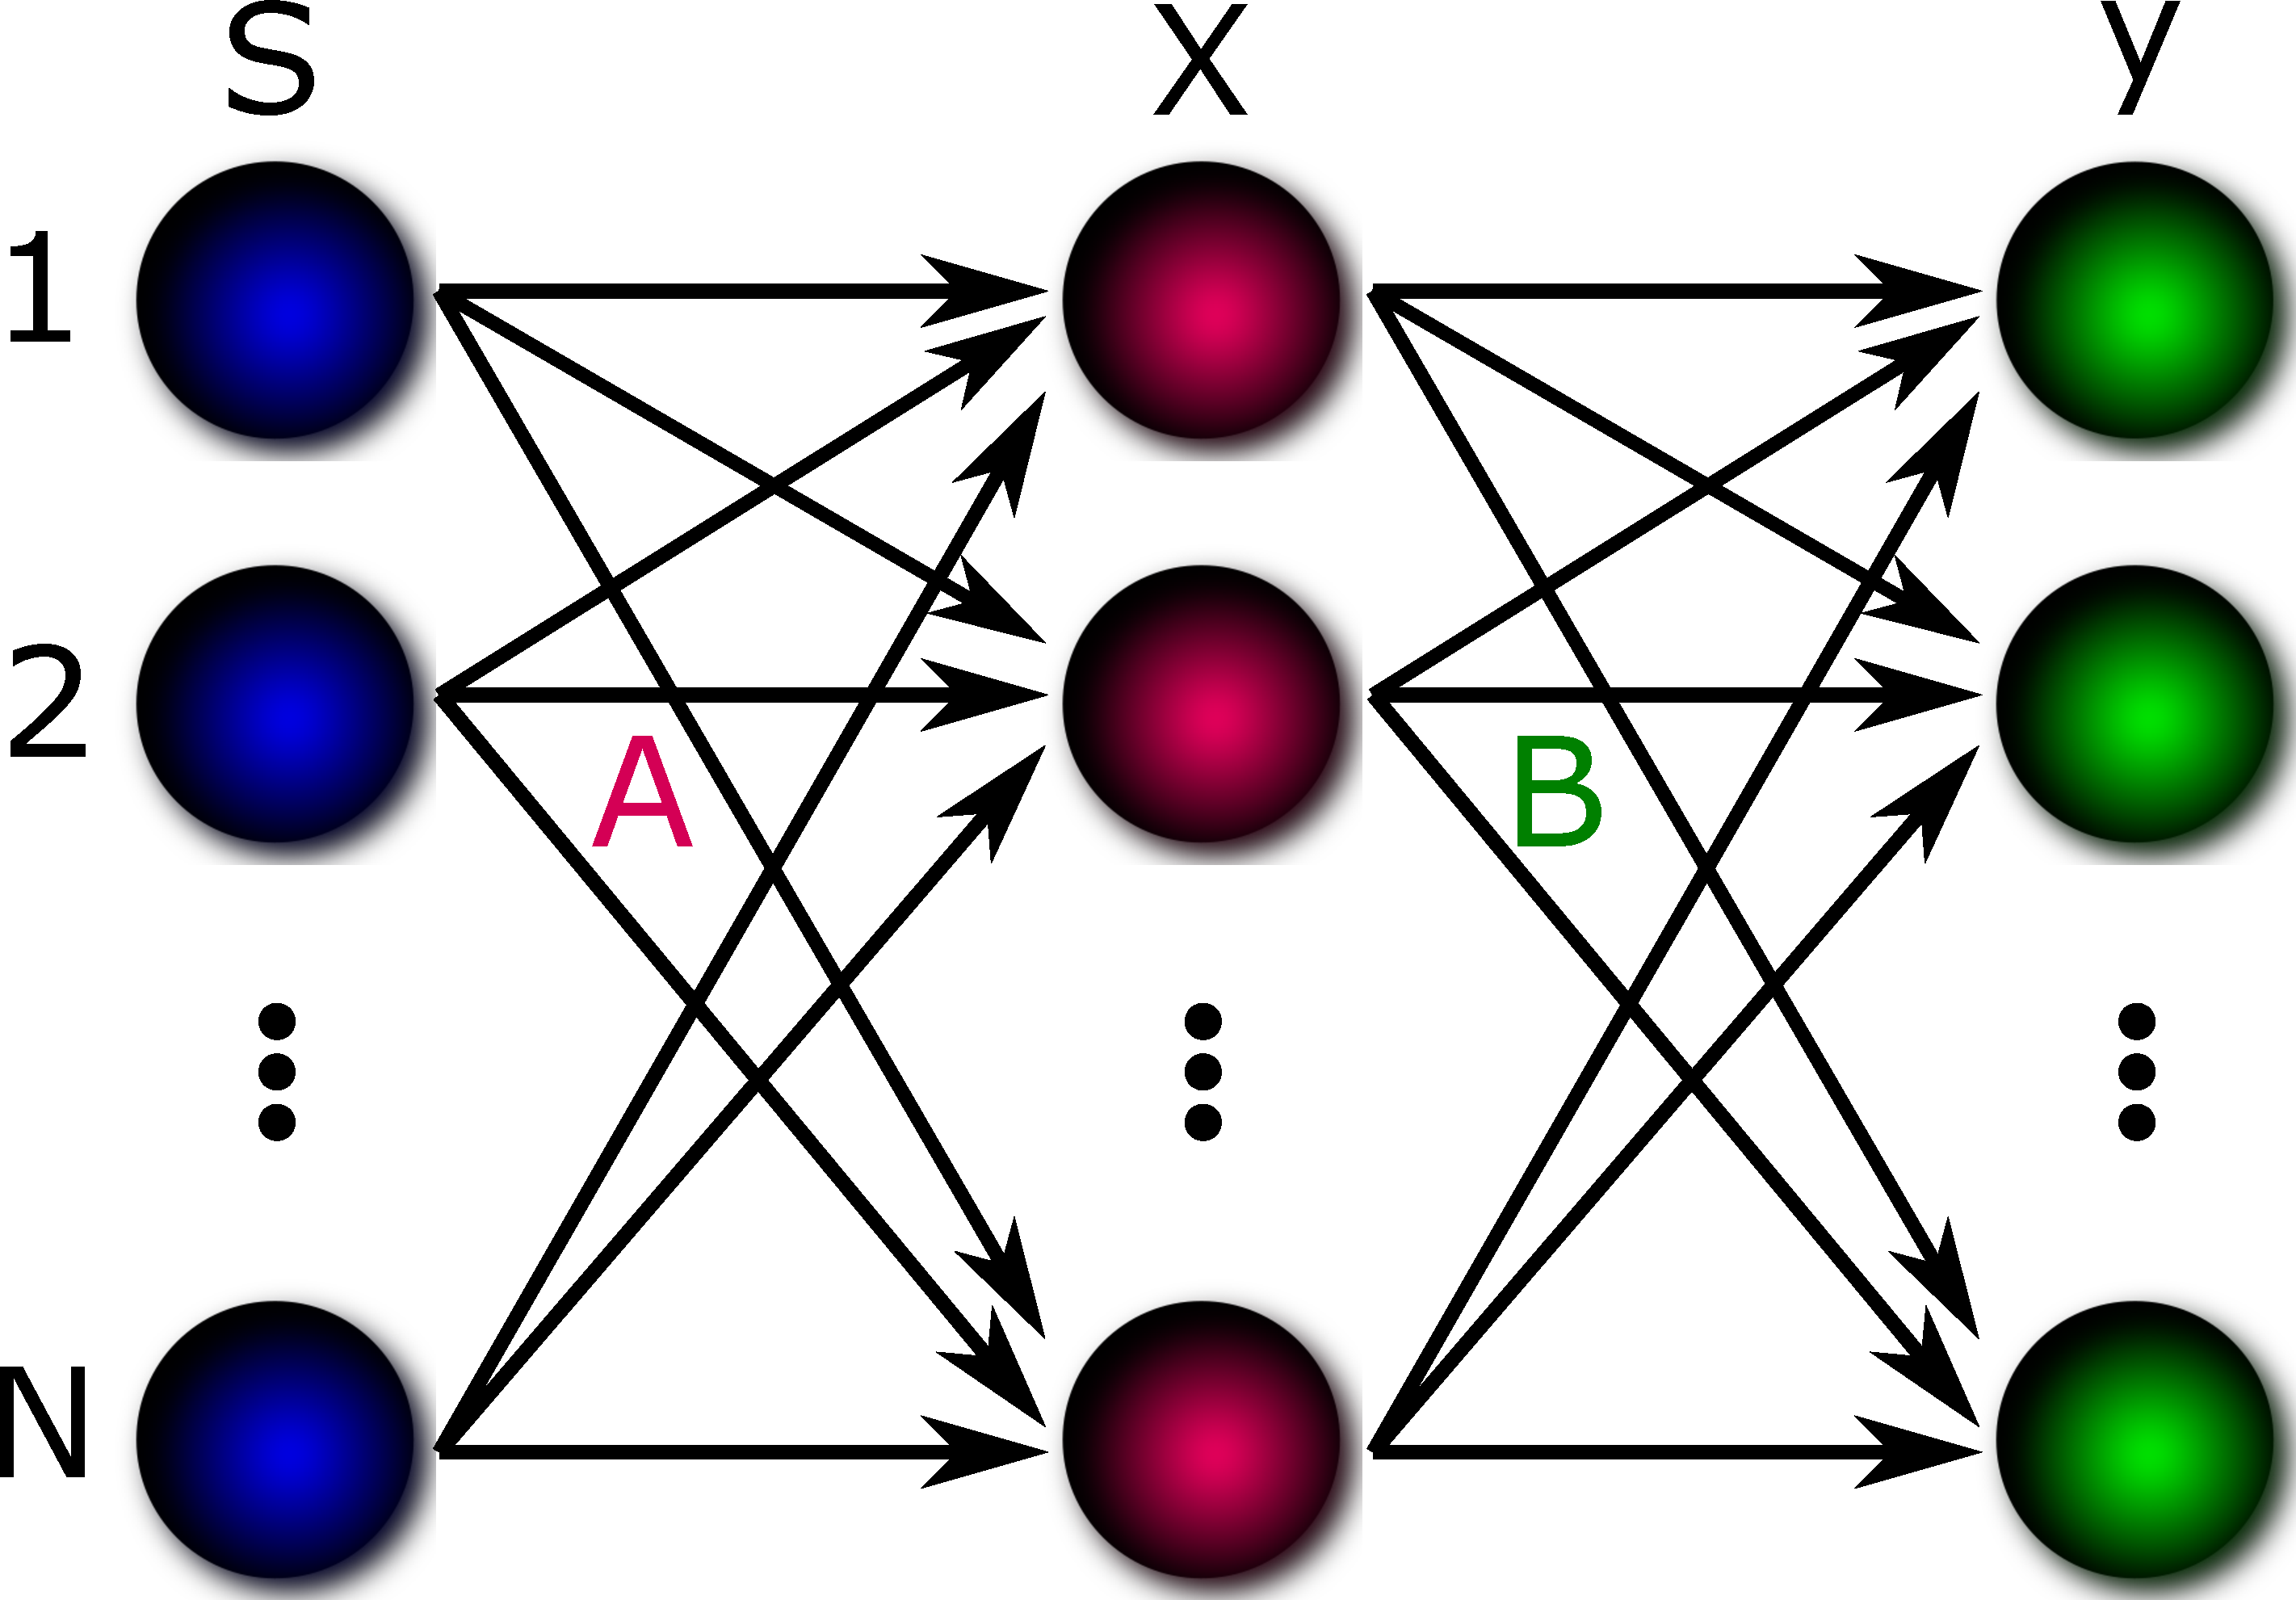
\includegraphics[width=0.40\textwidth]{figs/BSS.pdf}
    \caption{Uma representação genérica de um problema de BSS. $S$ é o conjunto de fontes originais, $X$ é o conjunto de sensores e $y$ é o conjunto de saídas após todo o processo de separação de sinais. $A$ representa a mistura do meio e do sensor em si; $B$, o processo de separação.}
    \label{fig:bss}
\end{figure}

A Figura \ref{fig:bss} ilustra um exemplo de problema geral de separação cega de fontes e pode ser usada para descrever esquematicamente uma ampla gama de diferentes aplicações. É importante lembrar que número de elementos em cada conjunto ($S$, $X$ e $y$) pode ser diferente, ou seja, dado há casos que podem envolver um número de fontes superior ao número de sensores, assim como o contrário também pode ocorrer. Ainda que houvesse apenas um único sensor compondo $X$ e um número enorme de fontes compondo $S$, por mais complexa que fosse a tarefa de separação, seria um caso possível e digno de ser interpretável como pertencente ao conjunto representado por tal ilustração.

% A Tabela \ref{tab:bss_examples} oferece alguns exemplos de diferentes cenários que poderiam ser esquematicamente abstraídos pela ilustração da Figura \ref{fig:bss}.

% \begin{table}[H]
%     \centering
%     \caption{Exemplos de diferentes cenários de BSS.}
%     \resizebox{\textwidth}{!}{%
%     \begin{tabular}{llll}
%     \toprule
%     \thead{Cenário}    &   \thead{$S$}   &   \thead{$X$}   &   \thead{$y$} \\
%     \midrule
%     \makecell[l]{Sinais cerebrais \\ coletados por um \\ arranjo de sensores}  & \makecell[l]{Diferentes partes \\ do cérebro}  & \makecell[l]{Mistura resultante \\ de sinais \\ cerebrais distintos}   & \makecell[l]{Sinais separados \\ de diferentes \\ partes do cérebro} \\

%     \makecell[l]{Sinais de \\ instrumentos \\ musicais coletados \\ por microfones}  & \makecell[l]{Instrumentos \\ musicais}  & \makecell[l]{Mistura de \\ sinais de \\ microfones}   & \makecell[l]{Sinais separados \\ de cada \\ instrumento} \\

%     \makecell[l]{Pessoas \\ conversando e \\ sendo gravadas \\ por microfones}  & \makecell[l]{Pessoas \\ conversando}  & \makecell[l]{Mistura de \\ sinais de \\ múltiplos \\ microfones}   & \makecell[l]{Sinais separados \\ de cada pessoa \\ falando} \\

%     \makecell[l]{Sistema de \\ comunicação \\ sem fio}  & \makecell[l]{Transmissor}  & \makecell[l]{Mistura de \\ sinais lida \\ pelo receptor}   & \makecell[l]{Sinais de interesse \\ apropriadamente \\ filtrados} \\

%     \bottomrule
%     \end{tabular}}
%     \label{tab:bss_examples}
% \end{table}

Do ponto de vista da disponibilidade de informação, o cenário mais complexo trata-se do caso em que $X$ é composto exclusivamente por um único sensor. Em um contexto de fontes de sinais de áudio, tal cenário é descrito como ``monoaural'' na literatura. Existem abordagens específicas para se trabalhar com tal cenário, mas esse não é o cenário a ser considerado neste trabalho.


Considere o cenário específico proposto na Figura \ref{fig:bass_example}, sobre uma situação usual de dois sinais sendo gravados por dois microfones. Em uma sala com os dois instrumentos musicais sendo tocados simultaneamente, ambos os microfones capturariam misturas resultantes compostas por variações de ambos os instrumentos musicais. Mas o resultado desejado seria um único sinal do violão e outro sinal único do piano. No cenário descrito, apesar de sua complexidade, quando a matriz da mistura é invertível, essa meta passa a ser plenamente alcançável.

\begin{figure}[H]
    \centering
    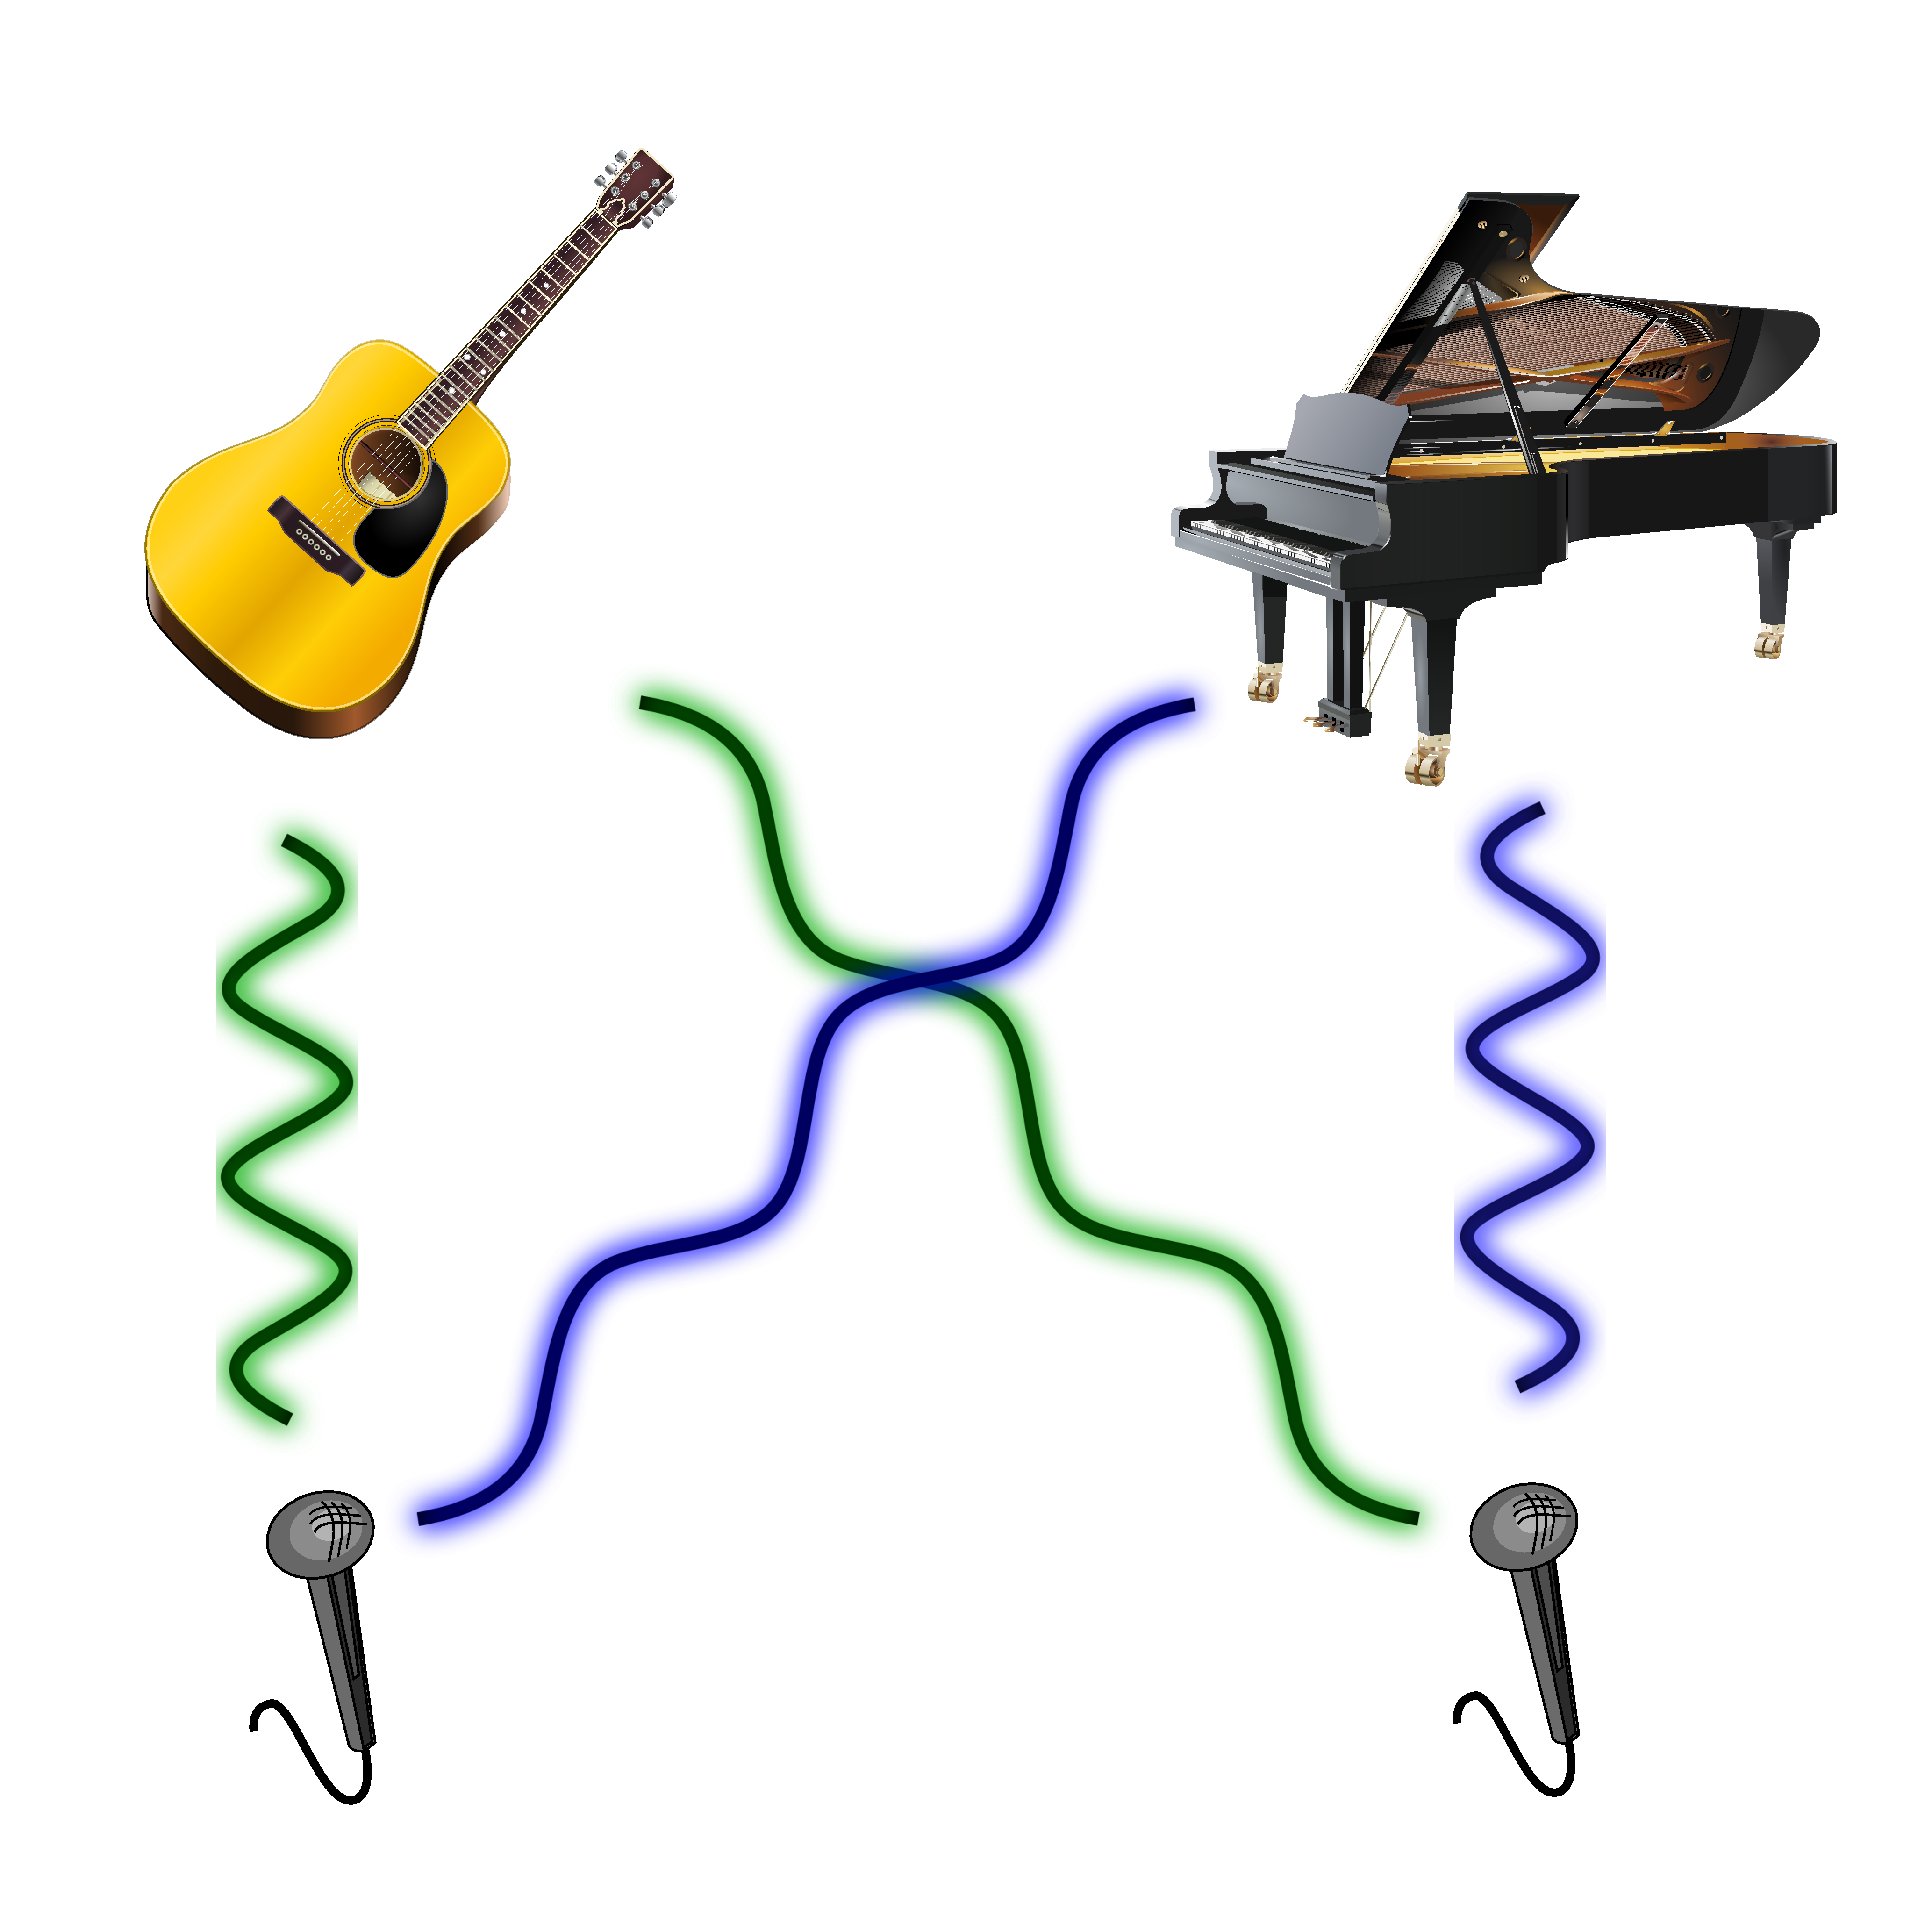
\includegraphics[width=0.60\textwidth]{figs/bass_example.pdf}
    \caption{Um exemplo típico de um problema BASS com múltiplos sinais de interesse e múltiplos microfones. Note que ambos os microfones gravam os sinais acústicos de ambos os instrumentos musicais, mas, devido ao fato de não serem microfones perfeitos, além de registrarem os ruídos do ambiente, introduzirão à mistura o seu próprio ruído característico.}
    \label{fig:bass_example}
\end{figure}

Existem várias técnicas diferentes que podem ser exploradas para alcançar um sinal resultante satisfatório para cada instrumento musical correspondente, por exemplo, o uso de informações tempo-frequenciais sobre cada instrumento musical envolvido e o uso de modelos probabilísticos para identificar as características desses sinais. Um bom trabalho explorando uma abordagem com múltiplos microfones foi feito em \citep{7805139}.

Se um dos microfones fosse removido, isso poderia ser interpretado erroneamente como uma variação simples do problema mostrado na Figura \ref{fig:bass_example}; a interpretação correta, na verdade, seria a de que trata-se de um problema totalmente diferente. Quando existem múltiplos microfones, um número maior de recursos está disponível, pois torna-se possível explorar características como distância relativa, o que contribui para facilitar o trabalho de separação de fontes.

É importante, no entanto, apontar para o fato de que esta seria uma perspectiva probabilística, ou seja, esta modelagem de problemas em particular exigiria uma análise não-determinística, o que geralmente requer um maior número de considerações e implicações, bem como aumentar a complexidade do problema, apesar de permitir uma análise muito mais flexível; dois exemplos de trabalhos que usaram essa abordagem monoaural são \citep{7194774}, que explorou Redes Neurais Recorrentes Profundas (\textbf{DRNN}, do inglês \textit{Deep Recurrent Neural Networks}), e \citep{7331633}, que usou a Fatoração de Matriz Não Negativa (\textbf{NMF}, do inglês \textit{Non-Negative Matrix Factorization}) Bayesiana.

\nomenclature{DRNN}{\textit{Deep Recurrent Neural Networks}}

A seguir serão trazidas algumas abordagens existentes sobre o uso de redes neurais e afins em um contexto de separação de fontes, oferecendo uma perspectiva histórica e exemplos de trabalhos marcantes da área.


%   ------------------------
%   ----- ANN para BSS -----
%   ------------------------
\section{Redes Neurais no contexto de BSS}
\label{sec:intro_ann_for_bss}

Existem diversas abordagens distintas para se realizar a tarefa de separação cega de fontes. Algumas delas exploram o uso de redes neurais, sobretudo quando há maior disponibilidade de poder computacional, mas a utilização de redes neurais em dois trabalhos não implica atacar o problema da mesma maneira em ambos os trabalhos. É importante que sejam consideradas as informações \textit{a priori}, a arquitetura da rede, as características exploradas, a presença ou ausência de rótulos para comparação, as técnicas de extração e seleção de características, as técnicas de validação cruzada, as métricas para aferição de desempenho etc.

Devido às suas propriedades generalistas, possivelmente interpretadas como um caráter positivo de ampla flexibilidade, as Redes Neurais Artificiais (\textbf{ANN}, do inglês \textit{Artificial Neural Networks}), que serão explicadas mais detalhadamente no Capítulo \ref{cha:ann}, podem oferecer um alto nível de efetividade na tarefa de separação cega de fontes, explicada na Seção \ref{sec:intro_bss} e mais detalhada no Capítulo \ref{cha:bss}. Tais características conferem às ANNs uma imensa abrangência quanto à sua gama de aplicações e a tarefa de separação de fontes pode ser muito beneficiada de tais qualidades; alguns exemplos interessantes serão discutidos ainda nesta seção.

\nomenclature{ANN}{\textit{Artificial Neural Networks}}

Um dos mais importantes trabalhos da área é \citep{herault1985detection}, que trouxe um conceito chamado \textit{computação de arquitetura neuromimética}\footnote{``Neuromimética'' pode ser interpretado como uma imitação do sistema (ou de partes do sistema) nervoso.}, que foi uma das essências do uso de redes neurais com a finalidade de separar sinais com base em uma abordagem de aprendizado não supervisionado.

Mais tarde, outro importante trabalho sobre separação de fontes foi publicado \citep{266878}, mas com enfoque na utilização de momentos de altas ordens\footnote{Em estatística, é comum entender como ordens superiores as ordens de grau igual ou maior que 3.} para isso. O trabalho reforçou a ideia de que a independência estatística dos sinais tratava-se de uma propriedade muito mais forte do que a sua mera descorrelação e, também, desde que fosse constatada uma diferença de distribuição entre os sinais envolvidos, seria possível identificar as assinaturas das fontes sem a dependência de quaisquer modelos \textit{a priori}, sendo que as tais assinaturas são autovetores da matriz de covariância após ter sido realizado um processo de ortonormalização e ponderação não linear.

O Algoritmo \ref{alg:intro_fobi} foi proposto para realizar a tarefa chamava-se FOBI (do inglês, \textit{\textbf{F}ourth-\textbf{O}rder \textbf{B}lind \textbf{I}dentification})

\nomenclature{FOBI}{\textit{Fourth Order Blind Identificiation}}

\noindent\begin{minipage}{\textwidth}
\renewcommand\footnoterule{}

\begin{algorithm}[H]
    \caption{FOBI (Fourth-Order Blind Identification) \citep{herault1985detection}.}
    \label{alg:intro_fobi}
    \begin{algorithmic}[1]

    \State Calcular a covariância:
    \begin{equation}
        R_{X} \leftarrow E\left(XX^{T}\right) \hspace{0.1cm},
        \label{eq:fobi_form_cov}
    \end{equation}

    \State Fatorar a covariância:
    \begin{equation}
        R_{X} = CC^{T} \hspace{0.1cm},
        \label{eq:fobi_fact_cov}
    \end{equation}

    \State Ortonormalizar os dados:
    \begin{equation}
        Y \leftarrow C^{-1}X \hspace{0.1cm},
        \label{eq:fobi_orto}
    \end{equation}

    \State Formar a covariância ponderada:
    \begin{equation}
        \widetilde{R}_{Y} \leftarrow E\left(\abs{Y}^{2}YY^{T}\right) \hspace{0.1cm},
        \label{eq:fobi_pond_cov}
    \end{equation}

    \State Extrair os autovetores da matriz de covariância:
    \begin{equation}
        \widetilde{R}_{Y} = \sum_{i=1}^{N} \left(\mu_{i} + N - 1\right) Y_{i} Y_{i}^{T} \hspace{0.1cm},
        \label{eq:fobi_eigen}
    \end{equation}

    \State Extrair as mensagens\footnote{Uma sequência de valores (dados) que pode carregar em si alguma informação, em um contexto de comunicação, geralmente é chamada de ``mensagem''.}:
    \begin{equation}
        \alpha_{i} \leftarrow Y_{i}^{T} Y \hspace{0.1cm},
        \label{eq:fobi_msg}
    \end{equation}

    \State Identificar as assinaturas\footnote{Assinatura pode ser entendida como o sinal original de informação advinda de uma dada fonte de comunicação.}:
    \begin{equation}
        X_{i} \leftarrow C Y_{i} \hspace{0.1cm}.
        \label{eq:fobi_sign}
    \end{equation}

    \end{algorithmic}

\end{algorithm}
\end{minipage}





%   ----- Aplicações Contemporâneas -----
\subsection{Aplicações Contemporâneas}
\label{subsec:contemp_app}

O trabalho \citep{7178348} utilizou-se de uma Rede Neural Profunda (\textbf{DNN}, do inglês \textit{Deep Neural Network}) para realizar um processo de extração de instrumentos musicais presentes em sinais resultantes de misturas musicais. Neste trabalho, a informação \textit{a priori} apenas assumiu conhecer os instrumentos que compunham as misturas, o que permitiu que um conjunto de dados de misturas para treinamento fosse construído a partir de trechos de áudio de sinais contendo exclusivamente instrumentos individuais, ou seja, misturas artificialmente produzidas. Fizeram parte das composições os seguintes instrumentos musicais: fagote, violoncelo, clarinete, chifre, piano, saxofone, trompete, viola e violino.

\nomenclature{DNN}{\textit{Deep Neural Network}}

A arquitetura explorada, que utilizou Unidade Linear Retificada (\textbf{ReLU}, do inglês \textit{Rectified Linear Unit}) \citep{nair2010rectified} como sua função de ativação, era composta por camadas intermediárias contendo o mesmo número de neurônios presentes na camada de saída, e a inicialização foi feita com base no algoritmo de mínimos quadrados. Foram consideradas como métricas a Relação Sinal-Distorção (\textbf{SDR}, do inglês \textit{Signal-to-Distortion Ratio}), a Relação Sinal-Interferência (\textbf{SIR}, do inglês \textit{Signal-to-Interference Ratio}), e a Relação Sinal-Artefato (\textbf{SAR}, do inglês \textit{Signal-to-Artifact Ratio}).

\nomenclature{ReLU}{\textit{Rectified Linear Unit}}
\nomenclature{SDR}{\textit{Signal-to-Distortion Ratio}}
\nomenclature{SIR}{\textit{Signal-to-Interference Ration}}
\nomenclature{SAR}{\textit{Signal-to-Artifact Ration}}

Este outro trabalho \citep{6245800} utilizou-se de uma combinação entre Análise de Componentes Independentes (\textbf{ICA}, do inglês \textit{Independent Component Analysis}) e redes neurais para realizar a separação cega de fontes ruidosas de sinais de voz em múltiplos canais, fazendo importantes considerações quanto aos ruídos associados durante todo o processo, inclusive pelo uso de redes neurais especificamente capazes de fazer tratamentos de remoção de ruídos dos sinais. A métrica de Relação Sinal-Ruído (\textbf{SNR}, do inglês \textit{Signal-to-Noise Ratio}) foi utilizada para se analisar o desempenho deste trabalho. É importante mencionar também a realização de duas etapas altamente influentes no desempenho obtido por este trabalho, que são: o branqueamento dos dados e a técnica \textit{Windage wipe off}.

\nomenclature{SNR}{\textit{Signal-to-Noise Ration}}



%   --------------------
%   ----- Desafios -----
%   --------------------
\section{Desafios}
\label{sec:intro_challenges}

Assim como ocorre em qualquer outra área do conhecimento, a área de separação de fontes possui os seus desafios. Conforme pesquisas na matemática, na ciência e na engenharia avançam, cada vez mais formas eficazes e eficientes são desenvolvidas para que esse objetivo possa ser atingido. Contudo, uma característica intrínseca da ciência é a sua incessante busca por respostas; e sabe-se que ao longo da busca pela resposta de uma pergunta, inevitavelmente, novas dúvidas serão encontradas, sendo que estas requererão novas buscas por respostas, preservando-se, então, tal apaixonante comportamento \textit{Ad infinitum}.

Novas dificuldades, novas barreiras, novos problemas e novas dúvidas sempre existirão. Por mais que se consiga vencer, transcender, resolver e responder, sempre haverá muito espaço novo a ser explorado por quem estiver interessado e for apto a desbravar-se nesse meio. As subseções a seguir trarão explanações acerca de alguns dos desafios mais comuns desta área.



%   ----- Subparametrizado -----
\subsection{Subparametrizado}
\label{subsec:intro_under-determined}

Um caso bastante corriqueiro desta área de pesquisa é conhecido como subparametrizado (ou, para fontes em inglês, \textit{Undetermined}), que consiste em um cenário cujo número de variáveis envolvidas é superior ao número de equações, impossibilitando que abordagens mais simples e diretas atinjam a eficácia desejada, pois, como se sabe, trata-se de um sistema com número infinito de soluções possíveis, o que está em desacordo com o que se almeja obter.

Para os fins deste trabalho, dado que as aplicações finais serão todas focadas em sinais de áudio, pode-se adaptar o uso de tais termos para uma linguagem mais próxima a tal área, de modo que a interpretação do problema se faça mais clara a partir de então. Assim sendo, o caso subparametrizado pode ser interpretado como sendo aquele em que o número de fontes de áudio é maior que o número de microfones.

Apenas para fins de exemplificação, poderia-se imaginar uma performance musical realizada por uma orquestra sendo gravada com um único microfone; a tarefa de separação neste caso seria subparametrizada, dado que seriam muitos instrumentos musicais a serem separados com base em um único sinal de uma mistura resultante do único microfone utilizado.




%   ----- Convolutivo -----
\subsection{Convolutivo}
\label{subsec:intro_convolutive}

Apesar de existir todo um conjunto de cenários mais simples, independentes de memória, modelos convolutivos, dependentes de memória, tendem a ser alternativas bastante convenientes para diversas aplicações, mas, como a complexidade do problema e o custo computacional tendem a crescer, cresce também a demanda por uma cautela extra no desenvolvimento dos modelos. A realização de processos de separação de fontes para cenários de misturas convolutivas pode ser feita por meio de técnicas com abordagens no domínio do tempo ou no domínio da frequência.




%   ----- Não-Linear -----
\subsection{Não-Linear}
\label{subsec:intro_non-linear}

Além de todas as possibilidades relacionadas a processos de misturas lineares, há também os casos de misturas não lineares, que são bem mais numerosas e complexas, embora sejam mais flexíveis e, assim, sejam capazes de causar efeitos ainda mais difíceis de serem desfeitos com elevados níveis de eficácia, o que pode demandar a utilização de técnicas mais rebuscadas e que ataquem o problema apartir de outras abordagens, tais como a análise de componentes independentes para misturas não lineares \citep{hyvarinen1999nonlinear}, misturas de tipo PNL \citep{taleb1999source} e processos de Gaussianização \citep{sole2003improving, ziehe2003blind}.



%   ---------------------------------------
%   ----- Nova Abordagem -- DNN e GAN -----
%   ---------------------------------------
\section{Nova Abordagem -- DNN e GAN}
\label{sec:intro_new_approach}

Após significativos avanços em redes neurais, tais como o desenvolvimento e o aprimoramento das redes de aprendizado profundas (\textit{Deep Learning}), assim como o surgimento da abordagem das GANs (\textit{Generative Adversarial Networks}) \citep{NIPS2014_5423}, que mostraram-se capazes de identificar e imitar padrões estatísticos em dados artificialmente gerados por elas próprias, começaram a surgir trabalhos que se utilizam de tais estruturas para realizar o processo de separação de fontes \citep{subakan2018generative, kaneko2018generative, fan2018svsgan}, o que chamou a atenção de parte da comunidade científica para o poder das GANs inclusive no que diz respeito à tarefa de separação de fontes, o que não havia sido especificamente trazido no trabalho original de Goodfellow em 2014, visto que os exemplos então apresentados eram todos ligados a aplicações voltadas para o processamento de imagens.


%   ---------------------
%   ----- Objetivos -----
%   ---------------------
\section{Objetivos}
\label{sec:intro_objectives}

Os principais objetivos perseguidos por este trabalho em particular são: a realização da tarefa de separação cega de fontes de áudio usando redes adversárias geradoras e o desenvolvimento de uma nova topologia baseada em seu modelo original.


%   ------------------------------------
%   ----- Estrutura da Dissertação -----
%   ------------------------------------
\section{Estrutura da Dissertação}
\label{sec:intro_dissertation_structure}

O Capítulo \ref{cha:bss}, intitulado ``Separação Cega de Fontes'', explicará alguns diferentes cenários, bem como aspectos e influências de linearidade e memória; também  serão expostos problemas relacionados e técnicas clássicas, que já são amplamente conhecidas e tipicamente utilizadas para realizar tarefas relacionadas ao problema de separação cega de fontes.

O Capítulo \ref{cha:ann} é reservado ao fornecimento de informações importantes sobre toda a base do que será explorado sobre Redes Neurais Artificiais ao longo deste trabalho, partindo de elementos históricos, passando pelas explicações sobre \textit{Perceptrons}, arquiteturas e propriedades, explanando a essência do \textit{Backpropagation} --um dos algoritmos mais importantes desta área-- e, finalmente, chegando às redes profundas, que são as que serão, de fato, utilizadas nos algoritmos deste trabalho.

O Capítulo \ref{cha:gan} explicará diversos aspectos sobre as Redes Adversárias Geradoras, desde sua origem, as bases de inspiração apoiadas em conceitos de teoria dos jogos, elementos estruturais, características intrínsecas desse modelo, alternativas para contornar problemas constatados e, por fim, aplicações em imagens, que, até então, é o tipo de mídia mais amplamente explorado quando tal ferramenta é utilizada.

O Capítulo \ref{cha:gan_for_bss} entrará no que, efetivamente, é o objetivo principal deste trabalho, i.e., a utilização de redes adversárias geradoras para a realização da tarefa de separação cega de fontes, que neste caso são sinais de áudio. Haverá uma seção destinada à explicação sobre como utilizar tal recurso. Também serão feitas diversas considerações relevantes, bem como uma ampla revisão bibliográfica contemporânea. Ao fim, serão discutidas as limitações identificadas e serão trazidas algumas propostas.

O Capítulo \ref{cha:results} trará uma série de simulações para diferentes cenários com suas respectivas metodologias explicadas, bem como resultados devidamente acompanhados de suas discussões.

O Capítulo \ref{cha:conclusion} encerrará o trabalho com as conclusões obtidas ao longo de todo este trabalho, bem como perspectivas futuras para possíveis caminhos a serem doravante trilhados.
